\documentclass[aspectratio=169]{beamer}
\usepackage[makeroom]{cancel}
\usepackage{verbatim}

\usepackage{bigints}

%\usepackage{unicode-math}
%\usepackage{mathtools}


\usepackage{listings}

%\usepackage{cmbright,fourier}

\newenvironment{metaverbatim}{\verbatim}{\endverbatim}

\usepackage{ulem}
\usepackage{mathtools}
%-=-=-=-=-=-=-=-=-=-=-=-=-=-=-=-=-=-=-=-=-=-=-=-=
%        LOADING PACKAGES
%-=-=-=-=-=-=-=-=-=-=-=-=-=-=-=-=-=-=-=-=-=-=-=-=
%\usepackage[utf8]{inputenc}
\usepackage{tikz}
\usepackage{amsmath}
\usepackage{amssymb}
\usepackage{natbib}
\usepackage[portuguese]{babel}
\usetikzlibrary{arrows}
\DeclareUnicodeCharacter{2212}{-}

\graphicspath{{images/}}

\usepackage{chronology}
\usepackage{multicol}
\usepackage{url}

              

\title{MS777 - Projetos supervisionados}
\author{{Gabriel Belém Barbosa}
}

\usepackage{amsmath}
\usepackage{amsthm}
\usepackage{amssymb}
\usepackage{amscd}
\usepackage{amsfonts}
\usepackage{amsbsy}
\usepackage{pdfpages}

\renewcommand\rmdefault{hpv}

%\usepackage{mathspec}
%\setmainfont{Gotham Book}
%\setmathrm{Gotham Book}
%\setmathfont(Digits,Latin){Gotham Book}


\newtheorem{lema}{Lema}
\BeforeBeginEnvironment{lema}{%
    \setbeamercolor{block title}{fg=white,bg=blue!50!black}
    \setbeamercolor{block body}{fg=black, bg=blue!10!white}
}

\newtheorem{corolario}{Corolário}
\BeforeBeginEnvironment{corolario}{%
    \setbeamercolor{block title}{fg=white,bg=orange!70!white}
    \setbeamercolor{block body}{fg=black, bg=orange!10!white}
}

\newtheorem{teorema}{Teorema}
\BeforeBeginEnvironment{teorema}{%
    \setbeamercolor{block title}{fg=white,bg=green!30!black}
    \setbeamercolor{block body}{fg=black, bg=green!20!white}
}


\newtheorem{exemplo}{Exemplo}
\BeforeBeginEnvironment{exercicio}{%
    \setbeamercolor{block title}{fg=white,bg=orange!85!black}
    \setbeamercolor{block body}{fg=black, bg=orange!20!white}
}


\newtheorem{exercicio}{Exercício}
\BeforeBeginEnvironment{exemplo}{%
    \setbeamercolor{block title}{fg=white,bg=red!70!black}
    \setbeamercolor{block body}{fg=black, bg=red!20!white}
}

\newtheorem{exerc}{Exercício}
\BeforeBeginEnvironment{exemplo}{%
    \setbeamercolor{block title}{fg=white,bg=red!70!black}
    \setbeamercolor{block body}{fg=black, bg=red!20!white}
}



\newtheorem{prova}{Prova}
\BeforeBeginEnvironment{prova}{%
    \setbeamercolor{block title}{fg=white,bg=red!70!black}
    \setbeamercolor{block body}{fg=black, bg=red!20!white}
}


\newtheorem{solucao}{Solução}
\BeforeBeginEnvironment{solucao}{%
    \setbeamercolor{block title}{fg=black,bg=yellow!85!black}
    \setbeamercolor{block body}{fg=black, bg=yellow!20!white}
}

\newtheorem{sol}{Solução}
\BeforeBeginEnvironment{solucao}{%
    \setbeamercolor{block title}{fg=black,bg=yellow!85!black}
    \setbeamercolor{block body}{fg=black, bg=yellow!20!white}
}

\def\C{\mathbb C}
\def\nx{\mathbf{x}}
\def\Z{\mathbb Z}
\def\N{\mathbb N}
\def\Q{\mathbb Q}
\def\H{\mathbb H}
\def\F{{\mathbb F}_q}
\def\cc{{\mathcal C}}
\def\bv{{\bf v}}
\def\rr{{\mathcal R}_n}
\def\im{{\bf i}}
\def\supp{\mathop{{\rm supp}}}
\def\zen{\mathop{\mathcal{Z}}}
\def\base{\mathcal{B}}
\def\Geny{\mathcal{G}}
\def\vezes{\mathop{{\rm times}}}
\def\Gal{\mathop{{\rm Gal}}}
\def\alge{\mathcal{A}}
\def\pr{\noindent{\sc proof. }}
\def\wh{\widehat}

%\def\lhd{\vartriangleleft}
%\newcommand{\fim}{\hspace*{\fill} $\square$\medskip}
%\newcommand{\ndv}{ \ {\mid \kern -0.70 em {\scriptstyle \not}} \ \ }

\newcommand{\rn}[1]{\mathbb{R}^{#1}}
\newcommand{\xpt}[1]{\dot{#1}}
\newcommand{\en}[1]{\textbf{e}_#1}
\newcommand{\ex}[1]{\noindent {\bf #1.}}
\newcommand{\zz}{\mathbb{Z}_{2}}

\newcommand{\bq}{\begin{equation}}
\newcommand{\e}{\varepsilon}
\newcommand{\T}{\theta}
\newcommand{\f}{\phi}
\newcommand{\eq}{\end{equation}}



\DeclareMathOperator{\sen}{sen}
\newcommand{\senx}{\sen(x)}

\newcommand{\bx}{{\bf x}}

\newcommand{\tr}{{\rm tr}}

\newcommand{\R}{\mathbb R}

\newcommand{\Rm}{\mathbb R^m}
\newcommand{\Rn}{\mathbb R^n}
\newcommand{\RR}{\mathbb R^2}
\newcommand{\RRR}{\mathbb R^3}



\usetheme{Boadilla}

\begin{document}

\begin{frame}{}
\maketitle
\end{frame}

%%%%%%%%%%%%%%%%%%%%%%
\begin{frame}{Introdução}
\begin{equation}
\label{eqn:og}
\dot{\mathbf{x}}=\left\{\begin{array}{ll}
\mathbf{A}^{+} \mathbf{x} & \text { se } x \geq 1 \\
\mathbf{A}^{-} \mathbf{x} & \text { se } x<1
\end{array}
\text{, }\mathbf{x}=
\begin{pmatrix}
x\\
y
\end{pmatrix}
\right.
\end{equation}\pause    
Trabalharemos o caso no qual $A^\pm$  possuem ambas um par de autovalores complexos, $\alpha^{\pm} \pm i \beta^{\pm}\text{, }(\beta^{\pm}>0\text{, } i^{2}=-1)$.
\end{frame}

\begin{frame}{Introdução}
É empregada a mudança de coordenadas $\mathbf{x} \rightarrow \mathbf{M^+ x}$, sendo
\[
\mathbf{M^+}=\left(\begin{array}{cc}
1 & 0 \\
m^+ & -n^+
\end{array}\right),
\] \pause 
onde $m^+$ e $n^+>0$ são tais que 
\[
\xi=\begin{pmatrix}
1\\
m^+ \pm in^+
\end{pmatrix}
\] 
são os autovetores de $\mathbf{A}^{+}$ associados a $\alpha^{+} \pm i \beta^{+}$, os autovalores da mesma.
\end{frame}

\begin{frame}{Introdução}
E o sistema (\ref{eqn:og}) é transformado em
    \begin{equation}
\label{eqn:jor}
\dot{\mathbf{x}}=\left\{\begin{array}{ll}
\mathbf{J}^{+} \mathbf{x} & \text { se } x \geq 1 \\
\mathbf{A}^{-} \mathbf{x} & \text { se } x<1
\end{array},\text{ }\mathbf{x}=\begin{pmatrix}
x\\
y
\end{pmatrix}\right.,
\end{equation}\pause
sendo $\mathbf{J}^{+}$ a forma normal de Jordan de $\mathbf{A}^{+}$,
\[
\mathbf{J}^{+}=\left(\begin{array}{cc}
\alpha^{+} & -\beta^{+} \\
\beta^{+} & \alpha^{+}
\end{array}\right).
\]\pause
Nomeando $\dot{\mathbf{x}}=\mathbf{J}^{+} \mathbf{x}$ seu subsistema direito e $\dot{\mathbf{x}}=\mathbf{A}^{-} \mathbf{x}$ seu subsistema esquerdo.
\end{frame}
\begin{frame}{Mapa de retorno de Poincaré}
    Denotando
\[
q^+(x, y)=\dot{x}=\alpha^+x − \beta^+y
\]
e
\[
q^-(x, y)=\dot{x}=a^−_{11}x + a^−_{12}y
\]
\end{frame}

\begin{frame}{Mapa de retorno de Poincaré}
E tomando
    \begin{equation}
\label{eqn:gmm}
q^+(1, \gamma^+)=\alpha^+ − \beta^+\gamma^+=0
\end{equation}
\[
\Rightarrow \gamma^+=\frac{\alpha^+}{\beta^+},
\]
\begin{equation}
\label{eqn:yc}
q^+(1, y_c^-)=a^−_{11} + a^−_{12} y_c^-=0
\end{equation}
\[
\Rightarrow y_c^-=-\frac{a^−_{11}}{a^−_{12}}.
\]
e
\[
\gamma^-=\frac{\alpha^-}{\beta^-}
\]
\end{frame}
\begin{frame}{Mapa de retorno de Poincaré}
São definidos os mapas de retorno de cada subsistema
    \begin{equation}
\label{left}
P^-:y_0\mapsto y_1\text{, }y_0\in[y_*^-, \infty)
\end{equation}
e
\begin{equation}
\label{right}
P^+:y_1\mapsto y_2\text{, }y_1\in(-\infty,y_*^+]
\end{equation}
que levam um ponto inicial na linha de corte ao primeiro ponto na linha de corte do fluxo a partir do ponto inicial com $t>0$.
\end{frame}
\begin{frame}{Mapa de retorno de Poincaré}
    Os pontos $(1,y_*^\pm)^T$ são definidos tendo que respeitar as restrições $y_*^-\geq y_c^-$ e $y_*^+\leq \gamma^+$, delimitando o que é chamada região de costura (região na qual $q^+(1,y)q^-(1,y)<0$).
\end{frame}

\begin{frame}{Mapa de retorno de Poincaré}
\begin{tabular}{cc}
\centering
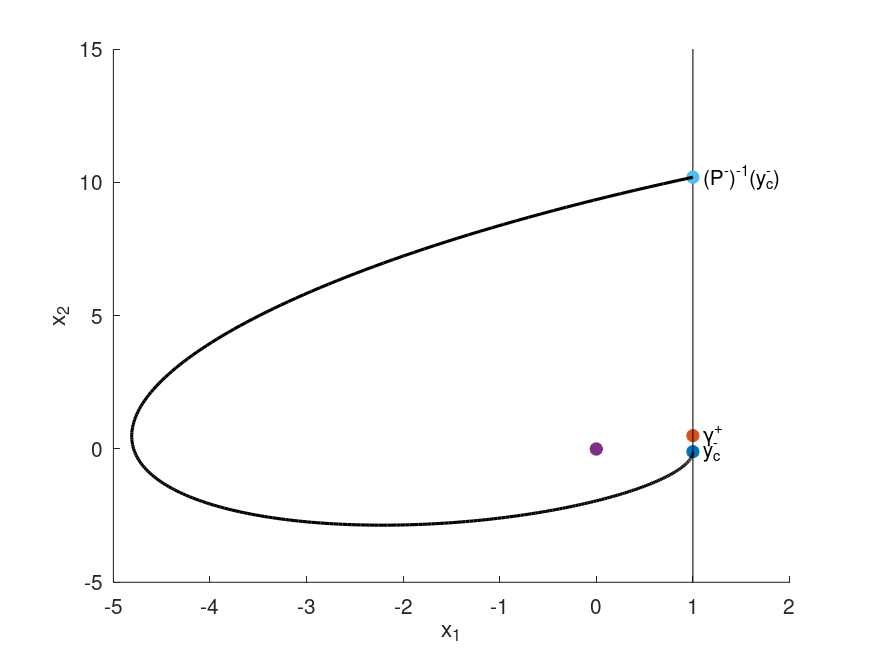
\includegraphics[width=6cm]{aaaaaa}
&
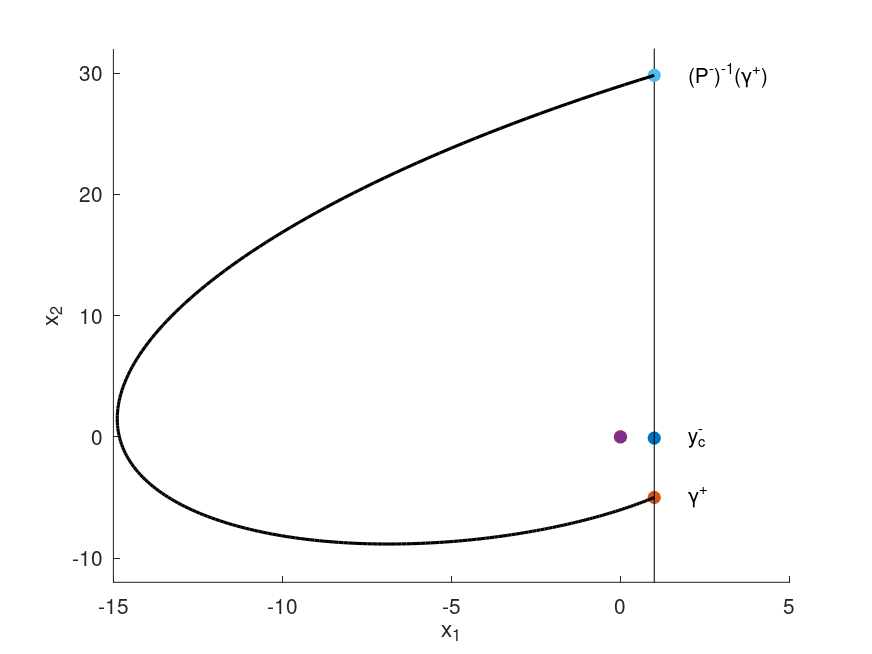
\includegraphics[width=6cm]{dddddd}\\
\small$\gamma^-<0$, $\gamma^+>y_c^-$&\small$\gamma^-<0$, $\gamma^+<y_c^-$
\end{tabular}
\end{frame}

\begin{frame}{Mapa de retorno de Poincaré}
\begin{tabular}{cc}
\centering
    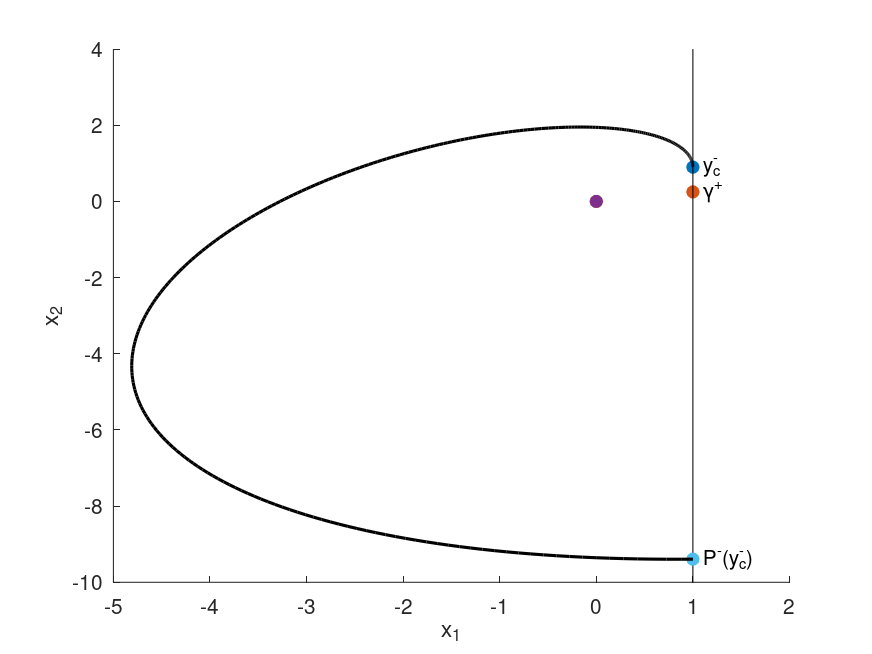
\includegraphics[width=6cm]{bbbbbb}
    &
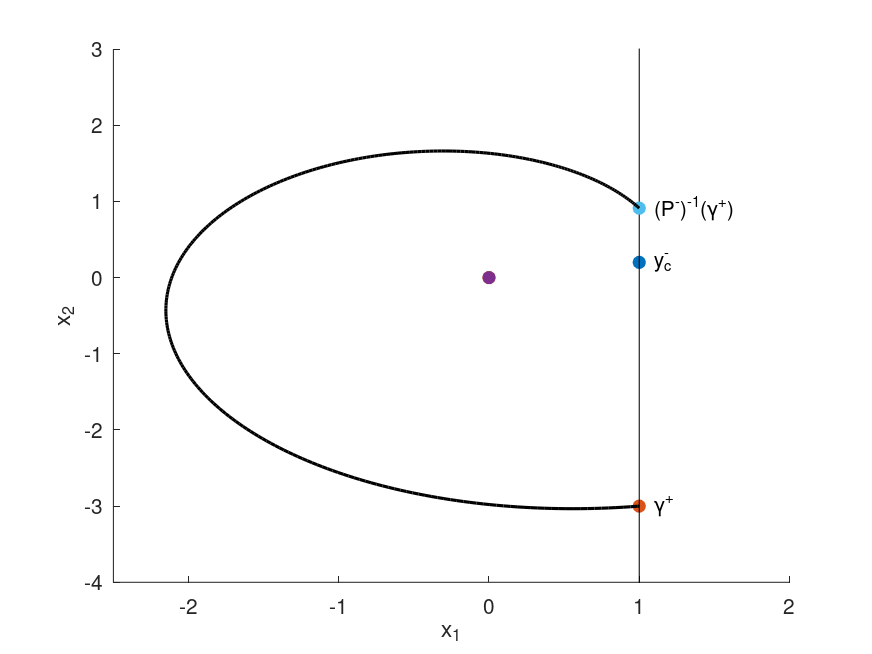
\includegraphics[width=6cm]{eeeeee}\\
\small$\gamma^->0$, $\gamma^+>y_c^-$&\small$\gamma^->0$, $P^-(y_c^-)>\gamma^+$
\end{tabular}
\end{frame}

\begin{frame}{Mapa de retorno de Poincaré}
    O mapa de retorno de Poincaré de (\ref{eqn:jor}) pode finalmente ser definido como
\begin{equation}
\label{eqn:poinc}
P=P^+\circ P^-: y_0\mapsto y_2\text{,  }y_0\in[y_*^-, \infty).
\end{equation}

\pause Um ciclo limite acontece quando $P(y_0)=y_0$ e é definido como uma órbita fechada isolada. De (\ref{eqn:poinc}), portanto, é evidente que um ciclo limite ocorre quando $P^-=(P^+)^{-1}$.
\end{frame}

\begin{frame}{Mapa de retorno de Poincaré}
    \begin{figure}
        \centering
        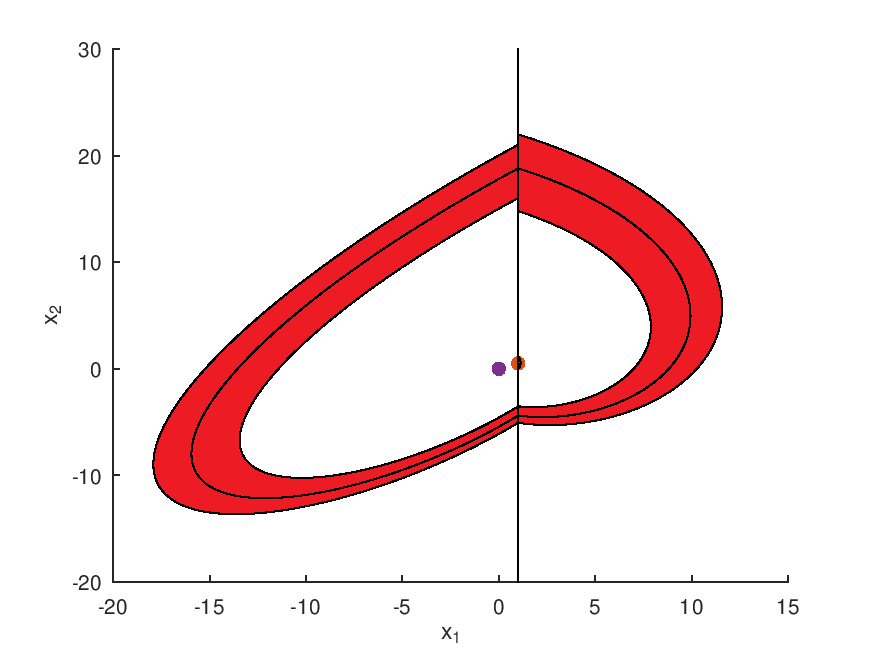
\includegraphics[width=6cm]{1_3_2}
        \caption{Exemplo de ciclo limite instável.}
        \label{fig:my_label}
    \end{figure}
\end{frame}

\begin{frame}{Mapa de retorno de Poincaré}
    Para aliviar a nomenclatura é definido
\begin{equation}
\label{phi}
\varphi_{\gamma}(\tau)=1-\exp (\gamma \tau) (\cos \tau-\gamma \sin \tau),
\end{equation}
e com operações elementares é útil definir $y_0/y_1$ e $y_1/y_2$ em função do tempo de voo entre eles, $\tau^{\pm}$.
\end{frame}

\begin{frame}{Mapa de retorno de Poincaré}
    Logo
\begin{equation}
\label{righttime}
\left\{\begin{array}{l}
y_{1}\left(\tau^{+}\right)=\gamma^{+}-\frac{\exp \left(-\gamma^{+} \tau^{+}\right) \varphi_{\gamma}+\left(\tau^{+}\right)}{\sin \tau^{+}}, \\
y_{2}\left(\tau^{+}\right)=\gamma^{+}+\frac{\exp \left(\gamma^{+} \tau^{+}\right)  \varphi_{-\gamma}+\left(\tau^{+}\right)}{\sin \tau^{+}}
\end{array}, \quad \tau^{+} \in(0, \pi)\right.,
\end{equation}

\begin{equation}
\label{lefttime}
\left\{\begin{array}{l}
y_{0}\left(\tau^{-}\right)=\frac{\beta^{-}}{a_{12}^{-}} \cdot \frac{\exp \left(-\gamma^{-} \tau^{-}\right)  \varphi_{\gamma^{-}}\left(\tau^{-}\right)}{\sin \tau^{-}}+y_{c}^{-}, \\
y_{1}\left(\tau^{-}\right)=-\frac{\beta^{-}}{a_{12}^{-}} \cdot \frac{\exp \left(\gamma^{-} \tau^{-}\right)  \varphi_{-\gamma^{-}}\left(\tau^{-}\right)}{\sin \tau^{-}}+y_{c}^{-}
\end{array}\right., \quad \tau^{-} \in\left(\pi, \hat{\tau}^{-}\right).
\end{equation}
\end{frame}

\begin{frame}{Mapa de retorno de Poincaré}
    Pela análise de (\ref{eqn:poinc}), foram obtidos resultados para o número de ciclos limite no plano $\gamma^+\times\gamma^-$ para $y^−_c=\gamma^+$, $y_c^-<\gamma^+$, e por invariância $y_c^->\gamma^+$. Porém o quadrante com $\gamma^+>0$, $\gamma^-<0$ do penúltimo caso e o quadrante com $\gamma^+<0$, $\gamma^->0$ do último, que são análogos entre si, não foram abordados e é o foco desse trabalho.
\end{frame}

\begin{frame}{Mapa de retorno de Poincaré}
    É possível construir uma matriz $A^-$ sob especificação como sendo
    \[
A^-=
\begin{pmatrix}
\alpha^--\frac{m^-\beta^-}{n^-}& \frac{\beta^-}{n^-}\\ 
-\beta^-\left(n^-+\frac{(m^-)^2}{n^-}\right)& \alpha^-+\frac{m^-\beta^-}{n^-}
\end{pmatrix},
\]\pause
com $m^-$ e $n^-$ definidos de forma análoga a suas contrapartes de $A^+$, por construção. Fixaremos $n^-=\alpha-$ para simplificar os cálculos.
\end{frame}

\begin{frame}{Mapa de retorno de Poincaré}
    Para satisfazer que a menor órbita seja um ciclo limite, ou seja, $P(y^-_*)=y^-_*$, sendo $y^-_*=(P^-)^{-1}(y^-_c)$ nesse caso, tem-se que, de (\ref{lefttime}) e (\ref{righttime})
$$
\left\{\begin{array}{l}
y_{c}^{-}=\gamma^{+}-\frac{\exp \left(-\gamma^{+} \hat{\tau}^{+}\right)  \varphi_{\gamma^{+}}\left(\hat{\tau}^{+}\right)}{\sin \left(\hat{\tau}^{+}\right)} \\
\frac{\beta^{-}}{a_{12}^{-}} \cdot \frac{\exp \left(-\gamma^{-} \hat{\tau}^{-}\right)  \varphi_{\gamma^{-}}\left(\hat{\tau}^{-}\right)}{\sin (\hat{\tau}^{-})}+y_{c}^{-}=\gamma^{+}+\frac{\exp \left(\gamma^{+} \hat{\tau}^{+}\right)  \varphi_{-\gamma^{+}}\left(\hat{\tau}^{+}\right)}{\sin \left(\hat{\tau}^{+}\right)}
\end{array}\right.,
$$\pause
sendo $\hat{\tau}^{+}$ o tempo de voo entre $y_c^-$ e  $y^-_*$ para o subsistema direito, e $\hat{\tau}^{-}$ o tempo de voo entre $y^-_*$ e $y_c^-$ para o subsistema esquerdo.
\end{frame}

\begin{frame}{Mapa de retorno de Poincaré}
    Da relação anterior é possível obter uma função erro em função de $\alpha^-$,
\begin{equation}
\label{zero}
f\left( \alpha^-\right)=\frac{1}{\hat{\tau}^-} \log\left(\frac{\sin(\hat{\tau}^-)a^-_{1,2}\left(exp(-\gamma^+\hat{\tau}^+)\varphi_{\gamma^{+}}\left(\hat{\tau}^{+}\right)+exp(\gamma^+\hat{\tau}^+)\varphi_{-\gamma^{+}}\left(\hat{\tau}^{+}\right)\right)}{\sin(\hat{\tau}^+)\beta^-\varphi_{\gamma^{-}}\left(\hat{\tau}^{-}\right)}\right)+\gamma^-,
\end{equation}\pause
onde $\hat{\tau}^\pm$ dependem de $\gamma^-$ e/ou $y_c^-$, logo dependem de $\alpha^-$, pela definição dos mesmos. Portanto é possível garantir a propriedade da menor órbita ser ciclo limite obtendo-se o zero de tal função erro. Segue, na Figura \ref{igua}, um exemplo de (\ref{eqn:jor}) obtido numericamente satisfazendo tal condição.
\end{frame}

\begin{frame}{Mapa de retorno de Poincaré}
    \begin{figure}[H]
\centering
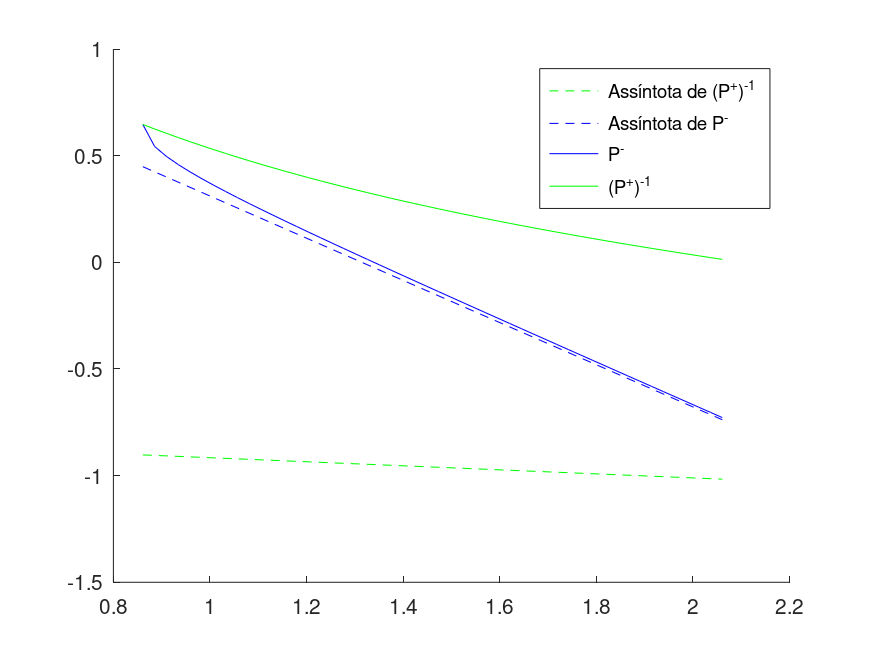
\includegraphics[width=8cm]{poinc}\\
\vspace{\baselineskip}
\caption{\label{igua}Gráfico de $P^-$ e $(P^+)^{-1}$ com $P(y^-_*)=y^-_*$.}
\end{figure}
\end{frame}

\begin{frame}{Mapa de retorno de Poincaré}
    Além disso (\ref{lefttime}) possui
    \begin{equation}
\label{assin}
 y_{1}=-\exp \left(\gamma^{-} \pi\right)  y_{0}+\frac{a_{22}^{-}}{a_{12}^{-}} \left[1+\exp \left(\gamma^{-} \pi\right)\right]
\end{equation}
como uma linha assintótica com  $y_{0} \to\infty$. \pause Dessa relação, $m^-$ será escolhido de forma que a linha assintótica de (\ref{lefttime}) seja valorada $c<\gamma^+$ em $y^-_*$, isto é, a assíntota passa pelo ponto $C=(y^-_*,c)^T$. De $A^-$
\begin{align*}
&\frac{a^-_{2,2}}{a^-_{1,2}}(1+exp(\gamma^-\pi))-exp(\gamma^-\pi)y_*^-=c \\
\Rightarrow&\left(\alpha^-\gamma^-+m^-\right)(1+exp(\gamma^-\pi))-exp(\gamma^-\pi)y_*^-=c \\
\Rightarrow& m^-=\frac{c+exp(\gamma^-\pi)y_*^-}{1+exp(\gamma^-\pi)}-\gamma^-\alpha^-.
\end{align*}
\end{frame}

\begin{frame}{Mapa de retorno de Poincaré}
É possível unir essa condição com a nulidade de (\ref{zero}), isto é, tendo como variável $\alpha^-$, em cada iteração da busca do zero desta última é efetuada uma busca do zero da função erro
\begin{equation}
\label{zero2}
g(m^-)=\frac{c+exp(\gamma^-\pi)y_*^-}{1+exp(\gamma^-\pi)}-\gamma^-\alpha^--m^-,
\end{equation}\pause
onde $y_*^-$ depende de $m^-$ e $\alpha^-$ é fixo. Na Figura \ref{c03} segue um exemplo de (\ref{eqn:jor}) obtido numericamente satisfazendo a nulidade de (\ref{zero}) e (\ref{zero2}) simultaneamente.
\end{frame}

\begin{frame}{Mapa de retorno de Poincaré}
    \begin{figure}[H]
\centering
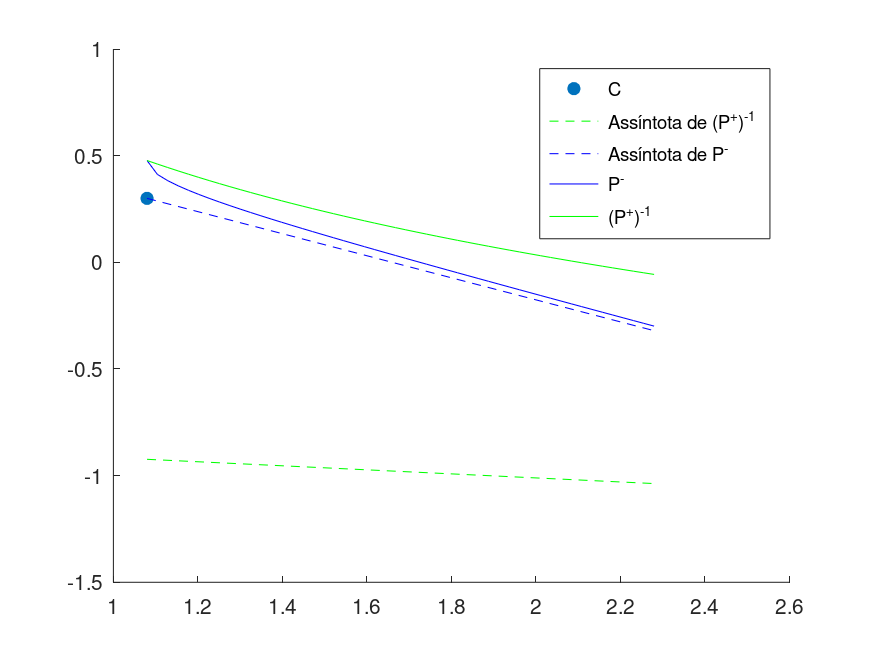
\includegraphics[width=8cm]{poinc3}\\
\vspace{\baselineskip}
\caption{\label{c03}Gráfico de $P^-$ e $(P^+)^{-1}$ com $P(y^-_*)=y^-_*$, $\gamma^+=0.75$, $\beta^-=1$ e $c=0.3$.}
\end{figure}
\end{frame}

\begin{frame}{Mapa de retorno de Poincaré}
    Sendo $\alpha^-_*$ o $\alpha^-$ tal que $y_c^-=\gamma^+$ (ou seja, um limitante para $\alpha^-$ visto que é trabalhado o caso $y_c^-<\gamma^+$), de (\ref{zero}) e (\ref{phi}), $\lim_{\alpha^-\to 0^-} f(\alpha^-)=\infty$, e $\lim_{\alpha^-\to (\alpha^-_*)^+} f(\alpha^-)=-\infty$, uma vez que $\lim_{\alpha^-\to (\alpha^-_*)^+}\hat{\tau}^+= 0$ da definição de $\hat{\tau}^+$. Logo existe $\alpha^-(\beta^-, c)\in(\alpha^-_*,0]$ tq. $f(\alpha^-)=0$, como pode ser visto na Figura \ref{curve}.
\end{frame}

\begin{frame}{Mapa de retorno de Poincaré}
    \begin{figure}[H]
\centering
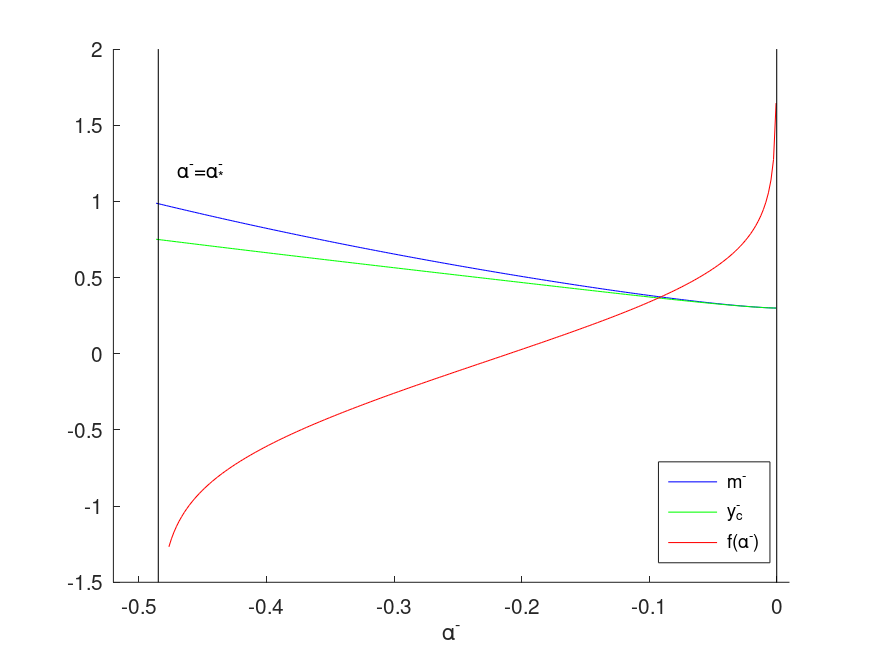
\includegraphics[width=8cm]{curve}\\
\vspace{\baselineskip}
\caption{\label{curve}Gráfico de $m^-$, $y_c^-$ e $f(\alpha^-)$ com $\gamma^+=0.75$, $\beta^-=1$ e $c=0.3$.}
\end{figure}
\end{frame}

\begin{frame}{Mapa de retorno de Poincaré}
    De (\ref{assin}), é possível notar que $\beta^-$ afeta a inclinação da assíntota de $P^-$ (e consequentemente o comportamento de $P$). Pautando-se no exemplo da Figura \ref{c03}, a Figura \ref{beta1} mostra um exemplo de (\ref{eqn:jor}) que ilustra o efeito da variação de $\beta^-$. 
\end{frame}

\begin{frame}{Mapa de retorno de Poincaré}
    \begin{figure}[H]
\centering
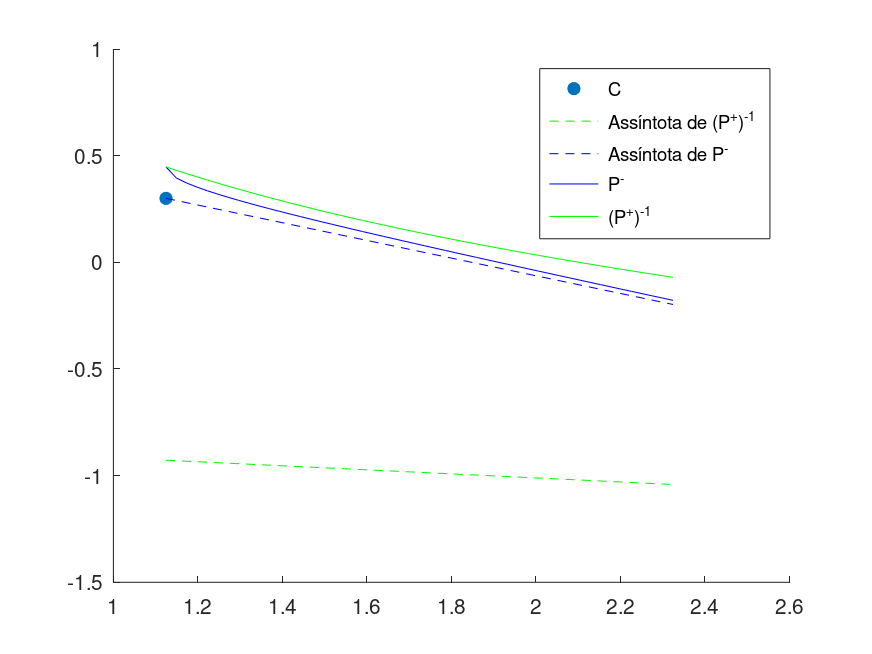
\includegraphics[width=8cm]{poinc2}\\
\vspace{\baselineskip}
\caption{\label{beta1}Gráfico de $P^-$ e $(P^+)^{-1}$ com $P(y^-_*)=y^-_*$, $\gamma^+=0.75$, $\beta^-=0.6$ e $c=0.3$.}
\end{figure}
\end{frame}

\begin{frame}{Mapa de retorno de Poincaré}
    Outra variável que pode ser inserida é uma folga $p$ em (\ref{zero}), de forma que ao se zerar a função ajustada com a folga, $P(y^-_*)\neq y^-_*$, porém de forma controlada. Para tal é criada a a função erro ajustada
\begin{equation}
\label{zero3}
f'\left( \alpha^-\right)=f\left( \alpha^-\right)+p,
\end{equation}
cujo efeito ao ser usada no lugar de $f\left( \alpha^-\right)$ pode ser observado na Figura \ref{folga}.
\end{frame}

\begin{frame}{Mapa de retorno de Poincaré}
    \begin{figure}[H]
\centering
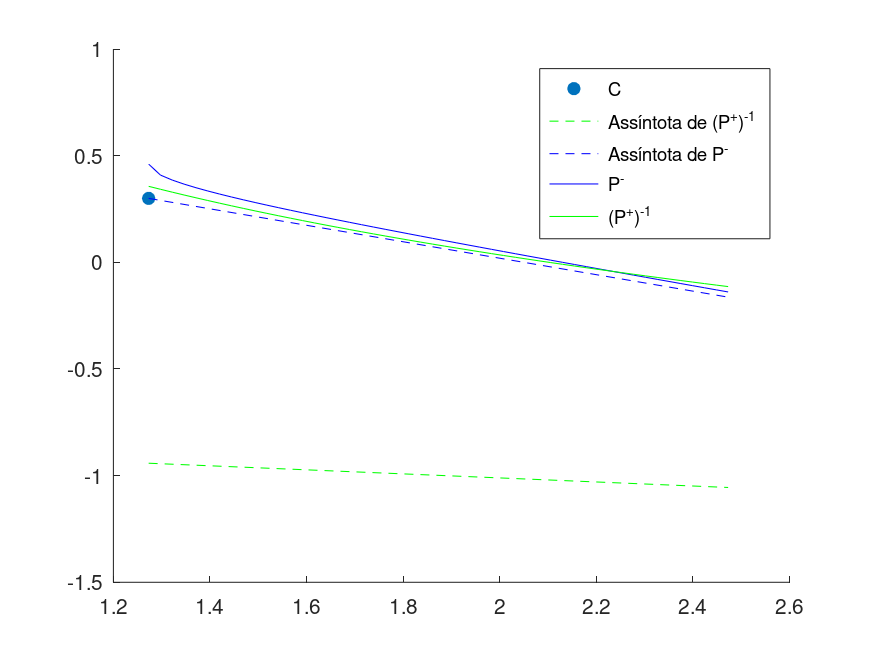
\includegraphics[width=8cm]{folga}\\
\vspace{\baselineskip}
\caption{\label{folga}Gráfico de $P^-$ e $(P^+)^{-1}$ com $f'\left( \alpha^-\right)=0$, $p=0.05$, $\gamma^+=0.75$, $\beta^-=0.6$ e $ c=0.3$.}
\end{figure}
\end{frame}

\begin{frame}{Mapa de retorno de Poincaré}
    Através das ideias apresentadas, pela forma das curvas de $P^-$ e $(P^+)^{-1}$, conjectura-se que dado um $\gamma^+>0$ qualquer, existe $ \beta^-(\gamma^+)>0$, $c(\gamma^+, \beta^-)<\gamma^+$ e $p(c, \gamma^+, \beta^-)$ tal que 3 ciclos limites se formam (com um exemplo fornecido na Seção 3), ou seja, que as curvas $P^-$ e $(P^+)^{-1}$ se intersectem 3 vezes. Contudo, estudos mais aprofundados do mapa de retorno $P$ ainda precisem ser efetuados para uma conclusão concreta.
\end{frame}

\begin{frame}{Resultados e conclusão}
    \begin{figure}[H]
\centering
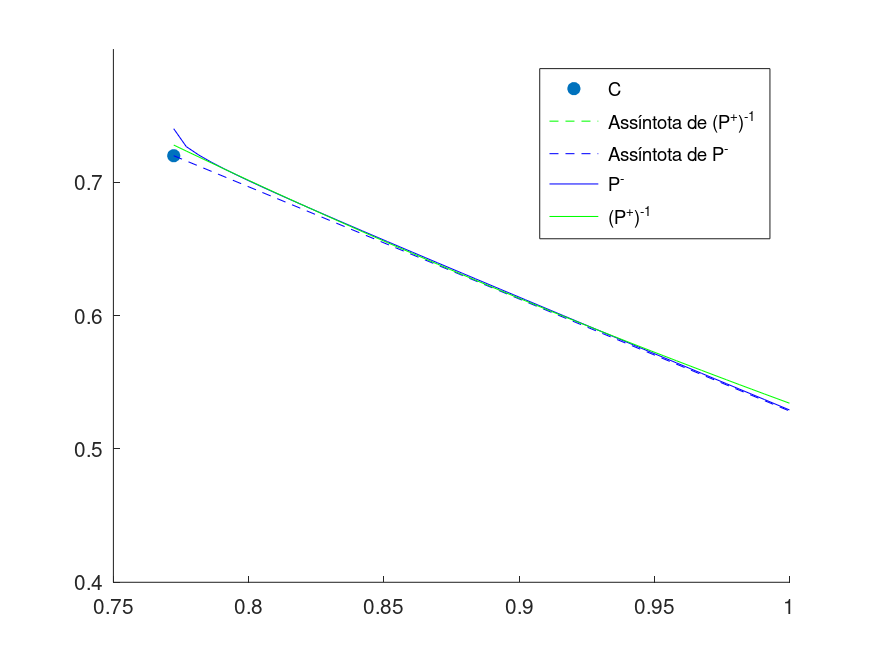
\includegraphics[width=8cm]{three}\\
\vspace{\baselineskip}
\caption{\label{three}Gráfico de $P^-$ e $(P^+)^{-1}$ com $f'\left( \alpha^-\right)=0$, $p=0.09$, $\gamma^+=0.75$, $\beta^-=0.6$ e $ c=0.72$.}
\end{figure}
\end{frame}

\begin{frame}{Resultados e conclusão}
    \begin{figure}[H]
\centering
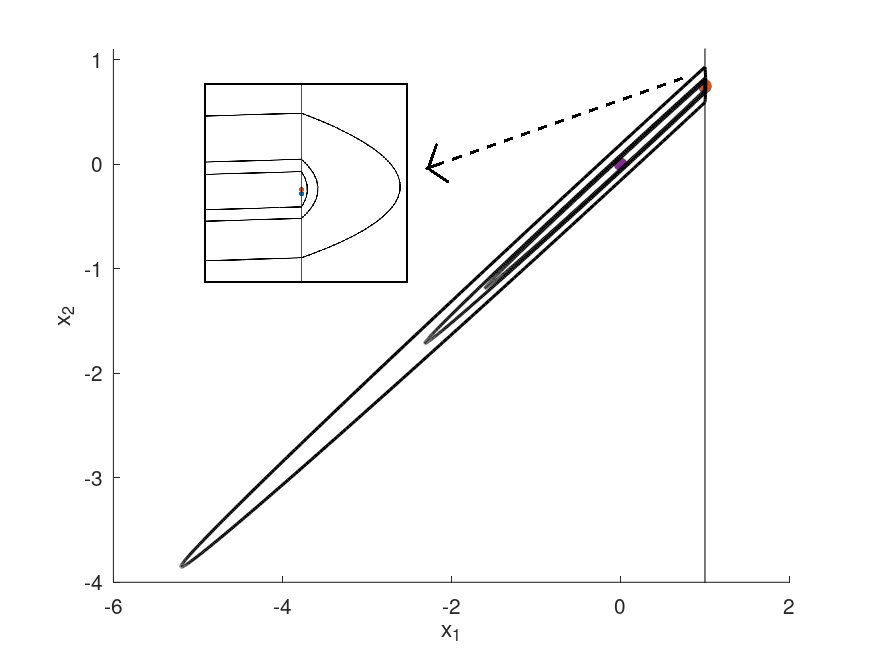
\includegraphics[width=8cm]{triz}\\
\vspace{\baselineskip}
\caption{\label{triz}Três ciclos limite a partir de $\gamma^+=0.75$.}
\end{figure}
\end{frame}

\begin{frame}{Referências}
\nocite{*}
\bibliographystyle{plainnat}
\footnotesize
\bibliography{monografia}
\end{frame}

\end{document}
